\documentclass[a4paper,article,14pt]{extarticle}

\usepackage{spbudiploma}
\usepackage{amsmath}
\usepackage{mathtools}
\usepackage[pdftex]{graphicx}
\graphicspath{{../pictures/}}
\usepackage{listings}
\usepackage{xcolor}
\usepackage{amsfonts}
\usepackage{amsmath}
\usepackage{cases}

\usepackage{enumitem}
\definecolor{codegreen}{rgb}{0,0.6,0}
\definecolor{codegray}{rgb}{0.5,0.5,0.5}
\definecolor{codepurple}{rgb}{0.58,0,0.82}
\definecolor{backcolour}{rgb}{0.95,0.95,0.92}

\lstdefinestyle{mystyle}{
	backgroundcolor=\color{backcolour},   
	commentstyle=\color{codegreen},
	keywordstyle=\color{codegreen},
	numberstyle=\tiny\color{codegray},
	stringstyle=\color{codepurple},
	basicstyle=\ttfamily\footnotesize,
	breakatwhitespace=false,         
	breaklines=true,                 
	captionpos=b,                    
	keepspaces=false,                 
	numbers=left,                    
	numbersep=5pt,                  
	showspaces=false,                
	showstringspaces=false,
	showtabs=false,                  
	tabsize=2
}

\lstset{style=mystyle}

\begin{document}
	\begin{titlepage}
		\begin{center}
			FEDERAL STATE AUTONOMOUS EDUCATIONAL INSTITUTION
			
			OF HIGHER EDUCATION
			
			ITMO UNIVERSITY
			\vspace{3cm}
			
			\large\textbf{Report}
			
			\large on the practical task No. 6
			
			\large \flqq Algorithms on graphs. \\ Path search algorithms on weighted graphs\frqq
			\vspace{5cm}
			

			\begin{flushright}
				{Performed by:} \\
				Putnikov Semyon \\ 
				J4132c \\
			\end{flushright}
			
			
			\begin{flushright}
				{Accepted by:} \\
				Dr Petr Chunaev \\ 
			\end{flushright}
			\vfill
			
			{St. Petersburg}
			\par{\number\year}
		\end{center}
	\end{titlepage}

	\newpage
	
	\section{Goal}
	The use of path search algorithms on weighted graphs (Dijkstra's, A* and Bellman-Ford algorithms).
	
	\section{Formulation of the problem}
	\begin{enumerate}[label=\Roman*]
		\item Generate a random adjacency matrix for a simple undirected weighted graph of 100 vertices and 500 edges with assigned random positive integer weights (note that the matrix should be symmetric and contain only 0s and weights as elements). Use Dijkstra's and Bellman-Ford algorithms to find shortest paths between a random starting vertex and other vertices. Measure the time required to find the paths for each algorithm. Repeat the experiment 10 times for the same starting vertex and calculate the average time required for the paths search of each algorithm. Analyse the results obtained.
		\item Generate a 10x10 cell grid with 30 obstacle cells. Choose two random non-obstacle cells and find a shortest path between them using A* algorithm. Repeat the experiment 5 times with different random pair of cells. Analyse the results obtained.
		\item Describe the data structures and design techniques used within the algorithms.
	\end{enumerate}
	
	\section{Brief theoretical part}
	\subsection{Dijkstra's algorithm}
	\textbf{Problem:} given a weighted graph (with positive weights) and a source vertex, find shortest paths from the source to all other vertices.
	
	\textbf{Main idea:} It generates a shortest path tree (SPT) with the source as a root, with maintaining two sets: one set contains vertices included in SPT, other set includes vertices not yet included in SPT. At every step, it finds a vertex which is in the other set and has a minimum distance from the source.
	
	\textbf{Time complexity} is $O(|V|^2)$.
	
	\subsubsection{Algorithm}
	\begin{itemize}
		\item Create an SPT set sptSet that keeps track of vertices included in SPT, i.e., whose minimum distance from source is calculated and finalized. Initially, this set is empty.
		\item Assign a distance value to all vertices in the input graph. Assign the distance value for the source vertex as 0. Assign the distance value for other vertices as $\infty$.
		\item While sptSet does not include all vertices:
		\begin{itemize}
			\item Pick a vertex $u \notin 2$ sptSet that has a minimum distance value.
			\item Include $u$ in sptSet.
			\item Update the distance values of all adjacent vertices of $u$. To update the distance values, iterate through all adjacent vertices. For every adjacent vertex $v$, if the sum of distance value of $u$ (from the source) and weight of edge $(u, v)$ is less than the distance value of $v$, then update the distance value of $v$.
		\end{itemize}
	\end{itemize}
	\subsection{Bellman-Ford algorithm}
	\textbf{Problem:} Given a weighted graph (possibly directed and with negative weights)
	and a source vertex $s$, find shortest paths from $s$ to all vertices in the graph.
	If a graph contains a negative cycle (i.e. a cycle whose edges sum to a negative
	value) that is reachable from $s$, then there is no shortest path: any path that has
	a point on the negative cycle can be made shorter by one more walk around
	the negative cycle. In such a case, Bellman–Ford can detect the negative cycle.
	
	\textbf{Note:} Dijkstra does not work for negative weights. Bellman-Ford is simpler than
	Dijkstra but its time complexity is $O(|V||E|)$.
	
	\textbf{Idea:} At i-th iteration, Bellman-Ford calculates the shortest paths which have at
	most $i$ edges. As there is maximum $|V| - 1$ edges in any simple path,
	$i = 1,...,|V| - 1$. Assuming that there is no negative cycle, if we have
	calculated shortest paths with at most $i$ edges, then an iteration over all edges
	guarantees to give shortest paths with at most $(i + 1)$ edges. To check if there
	is a negative cycle, make $|V|$-th iteration. If at least one of the shortest paths
	becomes shorter, there is such a cycle.
	
	\subsection{A* algorithm}
	\textbf{Problem:} given a weighted graph (with positive weights), a source vertex and a target vertex, find a shortest path from the source to the target.
	
	\textbf{Main idea:} At each iteration, A* determines how to extend the path basing on the cost of the current path from the source and an estimate of the cost required to extend the path to the target. Time complexity is $O(|E|)$.
	
	One gets Dijkstra’s algorithm if the above-mentioned estimate is skipped.
	
	Consider a grid with obstacles that can be represented as a weighted graph (vertices=cells, weighted edges=shortest paths and their lengths).
	
	\subsubsection{Algorithm}
	We are given a square grid with obstacles, a source cell $c_s$ and a target cell $c_t$. The aim is to reach $c_t$ (if possible) from $c_s$ as quickly as possible. 
	
	A* extends the path according to the value of $f(c_k) = g(c_k) + h(c_k)$, where $g$ measures the cost to move from $c_s$ to $c_k$ by the path generated and $h$ measures the cost to move from $c_k$ to $c_t$.
	
	
	
	\section{Results}
	%Present the results of solving the assigned problems, including graphs and tables, as well as a brief discussion of the results obtained (at most 4 pages)
	
	\begin{enumerate}[label=\Roman*]
		\item Bellman–Ford runs in $O(|V|*|E|)$ time. Dijkstra runs in $O(|V|^2)$ time. When we have dense graph $|E| \approx |V|^2$Bellman–Ford runs mush more slowly than Dijkstra. But now we have only $5\%$ edges of possible and Bellman–Ford runs slowly enough (maybe this is highly depend on implementation).
		\item A* its Dijkstra with heuristic technique. Highly depends from choice of heuristic. Great for tasks with a simple graph grid as in our case (simple heuristic function).
	\end{enumerate}

	\begin{figure}[h!]
		\centering
		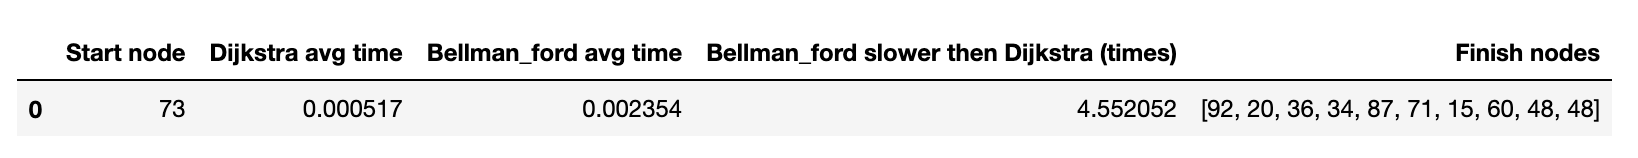
\includegraphics[scale=0.5]{results_1.png}
		\caption{Results of Dijkstra's and Bellman-Ford algorithms calculations.}
		\label{graph}
	\end{figure}


	\begin{figure}[h!]
		\centering
		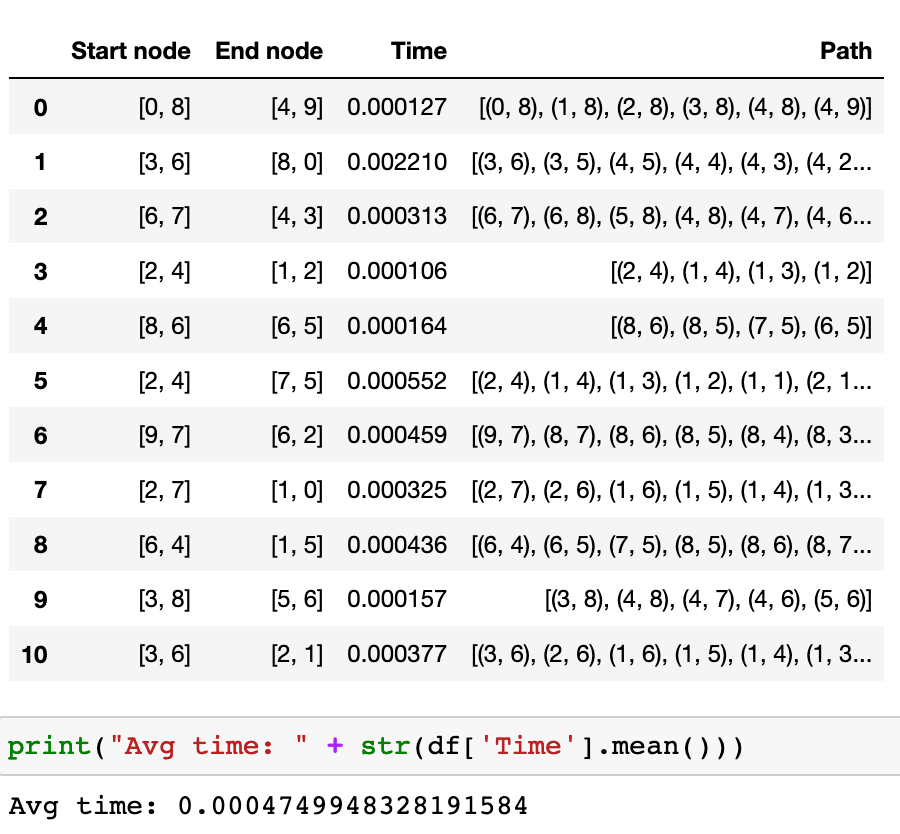
\includegraphics[scale=0.5]{results_2.png}
		\caption{Results of A* algorithm calculations.}
		\label{a}
	\end{figure} 
	
	I used dictionaries and lists for programming visualization of above algorithms. Also I used implementation of algorithms from python libs.

	
\end{document}